\documentclass[border=4pt]{standalone}
\usepackage{fontspec}
\setmainfont{DMSans9pt}[Path=../../fonts/, Extension=.ttf, UprightFont=*-Regular, BoldFont=*-Bold, ItalicFont=*-Italic, BoldItalicFont=*-BoldItalic]
\setsansfont{DMSans9pt}[Path=../../fonts/, Extension=.ttf, UprightFont=*-Regular, BoldFont=*-Bold, ItalicFont=*-Italic, BoldItalicFont=*-BoldItalic]
\usepackage{amsmath,amssymb,xcolor,adjustbox,pifont}
\usepackage{tikz}
\usetikzlibrary{arrows.meta,positioning,shapes.geometric,shapes.misc,fit,backgrounds,calc,decorations.pathreplacing,shadows}
\usepackage[edges]{forest}
\usepackage{pgfplots}
\pgfplotsset{compat=1.18}

%% ---------- colours and macros used throughout
\definecolor{cTwo}{HTML}{4C72B0}   % two-stage
\definecolor{cOne}{HTML}{DD8452}   % one-stage / YOLO
\definecolor{cDetr}{HTML}{55A868}  % DETR
\definecolor{cOvd}{HTML}{8172B3}   % open-vocabulary
\definecolor{cAgent}{HTML}{C44E52} % agentic
\definecolor{cEdge}{HTML}{937860}  % edge
\definecolor{cApp}{HTML}{DA8BC3}   % applications
\definecolor{cData}{HTML}{4C9BB0}  % data / metrics
\newcommand{\tleaf}[1]{\parbox{8.3cm}{\raggedright #1}}
\newcommand{\tmid}[1]{\parbox{2.9cm}{\raggedright #1}}
\newcommand{\tone}[1]{\parbox{2.3cm}{\raggedright #1}}
\newcommand{\cmark}{\ding{51}}
\newcommand{\xmark}{\ding{55}}
\newcommand{\pmark}{$\circ$}


\renewcommand{\cite}[1]{}
\providecommand{\ref}[1]{}
\renewcommand{\ref}[1]{}
\newcommand{\tbd}[1]{#1}
\begin{document}
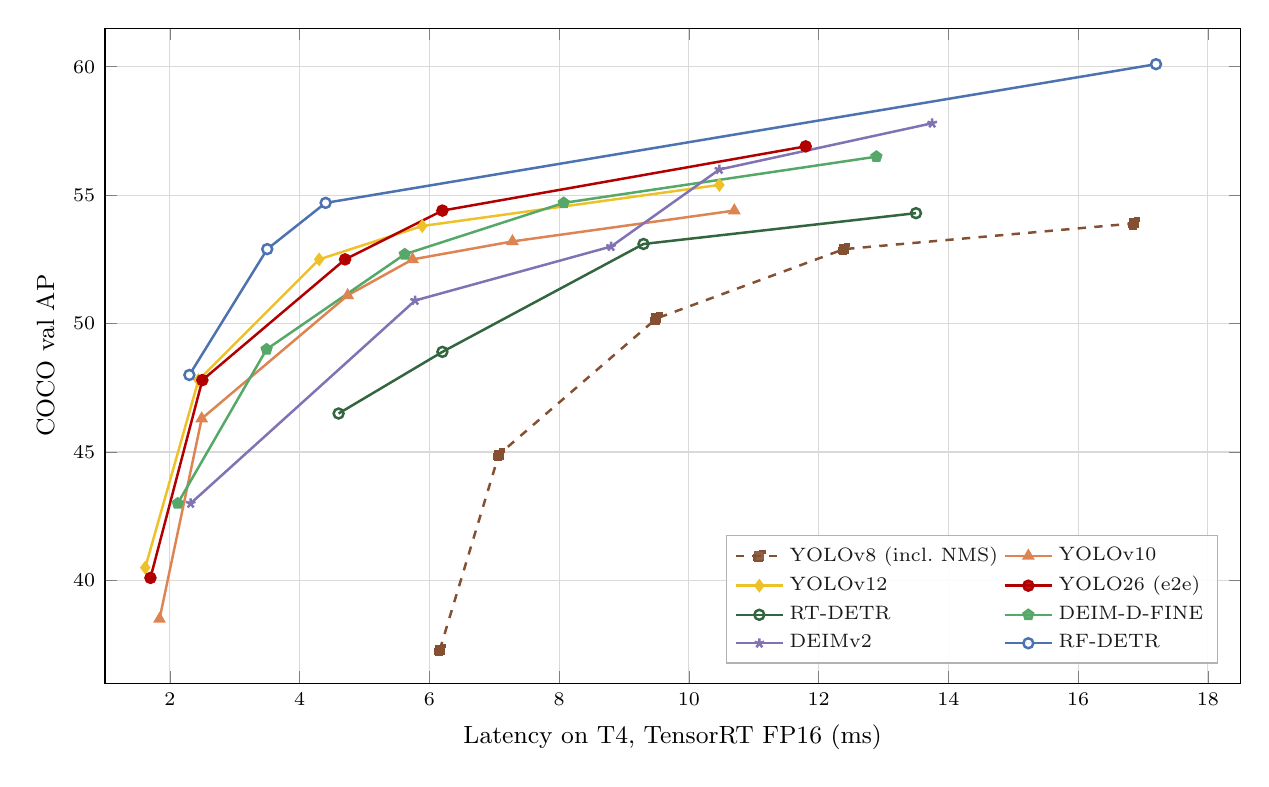
\begin{tikzpicture}
\begin{axis}[
  width=16cm, height=9.9cm,
  xlabel={Latency on T4, TensorRT FP16 (ms)}, ylabel={COCO val AP},
  xmin=1, xmax=18.5, ymin=36, ymax=61.5,
  grid=both, grid style={black!8}, major grid style={black!15},
  tick label style={font=\scriptsize}, label style={font=\small},
  legend style={font=\scriptsize, at={(0.98,0.03)}, anchor=south east, cells={anchor=west}, fill=white, fill opacity=0.9, draw=black!30},
  legend columns=2,
  every axis plot/.append style={line width=0.9pt, mark size=1.8pt},
]
\addplot[color=cOne!60!black, mark=square*, dashed] coordinates {(6.16,37.3)(7.07,44.9)(9.50,50.2)(12.39,52.9)(16.86,53.9)};
\addlegendentry{YOLOv8 (incl.\ NMS)}
\addplot[color=cOne, mark=triangle*] coordinates {(1.84,38.5)(2.49,46.3)(4.74,51.1)(5.74,52.5)(7.28,53.2)(10.70,54.4)};
\addlegendentry{YOLOv10}
\addplot[color=cOne!50!yellow, mark=diamond*] coordinates {(1.62,40.5)(2.44,47.8)(4.30,52.5)(5.89,53.8)(10.47,55.4)};
\addlegendentry{YOLOv12}
\addplot[color=red!70!black, mark=*] coordinates {(1.7,40.1)(2.5,47.8)(4.7,52.5)(6.2,54.4)(11.8,56.9)};
\addlegendentry{YOLO26 (e2e)}
\addplot[color=cDetr!60!black, mark=o] coordinates {(4.6,46.5)(6.2,48.9)(9.3,53.1)(13.5,54.3)};
\addlegendentry{RT-DETR}
\addplot[color=cDetr, mark=pentagon*] coordinates {(2.12,43.0)(3.49,49.0)(5.62,52.7)(8.07,54.7)(12.89,56.5)};
\addlegendentry{DEIM-D-FINE}
\addplot[color=cOvd, mark=star] coordinates {(2.32,43.0)(5.78,50.9)(8.80,53.0)(10.47,56.0)(13.75,57.8)};
\addlegendentry{DEIMv2}
\addplot[color=cTwo, mark=*, mark options={fill=white}] coordinates {(2.3,48.0)(3.5,52.9)(4.4,54.7)(17.2,60.1)};
\addlegendentry{RF-DETR}
\end{axis}
\end{tikzpicture}
\end{document}
